\documentclass[11pt,letterpaper]{article}

\usepackage[margin=0.72in]{geometry}
\usepackage[T1]{fontenc}
\usepackage[utf8]{inputenc}
\usepackage{lmodern}
\usepackage{graphicx}
\usepackage{xcolor}
\usepackage{booktabs}
\usepackage{tabularx}
\usepackage{longtable}
\usepackage{array}
\usepackage{enumitem}
\usepackage{hyperref}
\usepackage{fancyhdr}
\usepackage{titlesec}
\usepackage{caption}
\usepackage{float}
\usepackage{tikz}
\usetikzlibrary{arrows.meta,positioning,shapes.geometric,shapes.misc}
\graphicspath{{../}}

\definecolor{clinicGreen}{HTML}{12332C}
\definecolor{clinicGreen2}{HTML}{0F3F36}
\definecolor{clinicGold}{HTML}{F2C14E}
\definecolor{clinicMint}{HTML}{E8F6EF}
\definecolor{clinicInk}{HTML}{101828}
\definecolor{clinicMuted}{HTML}{475467}
\definecolor{clinicLine}{HTML}{D0D5DD}
\definecolor{clinicDanger}{HTML}{B42318}

\hypersetup{
  colorlinks=true,
  linkcolor=clinicGreen,
  urlcolor=clinicGreen2,
  citecolor=clinicGreen
}

\pagestyle{fancy}
\fancyhf{}
\lhead{\textcolor{clinicGreen}{Clinic Copilot BD}}
\rhead{\textcolor{clinicMuted}{Health Worker Assistant}}
\cfoot{\thepage}
\renewcommand{\headrulewidth}{0.4pt}
\renewcommand{\headrule}{\hbox to\headwidth{\color{clinicGold}\leaders\hrule height \headrulewidth\hfill}}

\titleformat{\section}{\Large\bfseries\color{clinicGreen}}{\thesection}{0.7em}{}
\titleformat{\subsection}{\large\bfseries\color{clinicGreen2}}{\thesubsection}{0.6em}{}
\titleformat{\subsubsection}{\normalsize\bfseries\color{clinicInk}}{\thesubsubsection}{0.5em}{}
\setlist[itemize]{leftmargin=1.3em,itemsep=0.2em,topsep=0.35em}
\setlist[enumerate]{leftmargin=1.4em,itemsep=0.2em,topsep=0.35em}
\captionsetup{font=small,labelfont=bf}

\newcommand{\pill}[1]{%
  \fcolorbox{clinicLine}{clinicMint}{\strut\hspace{0.5em}\textbf{\textcolor{clinicGreen}{#1}}\hspace{0.5em}}%
}

\newcommand{\callout}[2]{%
  \vspace{0.55em}
  \noindent\fcolorbox{clinicLine}{#1}{%
    \begin{minipage}{0.965\linewidth}
      \vspace{0.55em}
      #2
      \vspace{0.55em}
    \end{minipage}
  }
  \vspace{0.55em}
}

\newcommand{\screenshot}[3]{%
  \begin{figure}[H]
    \centering
    \includegraphics[width=\linewidth]{#1}
    \caption{#2}
    \small\textcolor{clinicMuted}{#3}
  \end{figure}
}

\newcommand{\membercard}[4]{%
  \noindent\fcolorbox{clinicLine}{white}{%
    \begin{minipage}{0.965\linewidth}
      \vspace{0.45em}
      \textbf{\textcolor{clinicGreen}{#1}} \hfill \textcolor{clinicMuted}{#2}\\
      \textcolor{clinicInk}{#3}\\
      \small\textcolor{clinicMuted}{#4}
      \vspace{0.45em}
    \end{minipage}
  }
  \vspace{0.45em}
}

\newcolumntype{Y}{>{\raggedright\arraybackslash}X}
\newcolumntype{L}[1]{>{\raggedright\arraybackslash}p{#1}}

\begin{document}

\begin{titlepage}
  \pagecolor{clinicGreen}
  \color{white}
  \vspace*{0.25in}
  \begin{minipage}{0.18\linewidth}
    
\includegraphics[width=0.86in]{artifacts/health-worker-latex-main/huntriox-logo.png}
  \end{minipage}
  \hfill
  \begin{minipage}{0.18\linewidth}
    \raggedleft
    
\includegraphics[width=0.82in]{artifacts/health-worker-latex-main/project-logo.svg.png}
  \end{minipage}
  \vspace{0.18in}
  {\Huge\bfseries Clinic Copilot BD\par}
  \vspace{0.22in}
  {\Large Health Worker Assistant for Bangladesh Frontline Care\par}
  \vspace{0.18in}
  {\large AI decision support for small hospitals, overloaded clinics, field health workers, and low-resource primary care teams\par}
  \vspace{0.32in}
  \pill{Local or cloud AI}
  \hspace{0.35em}
  \pill{MCP-ready}
  \hspace{0.35em}
  \pill{Human review}
  \hspace{0.35em}
  \pill{Bangla-first workflow}
  \vfill
  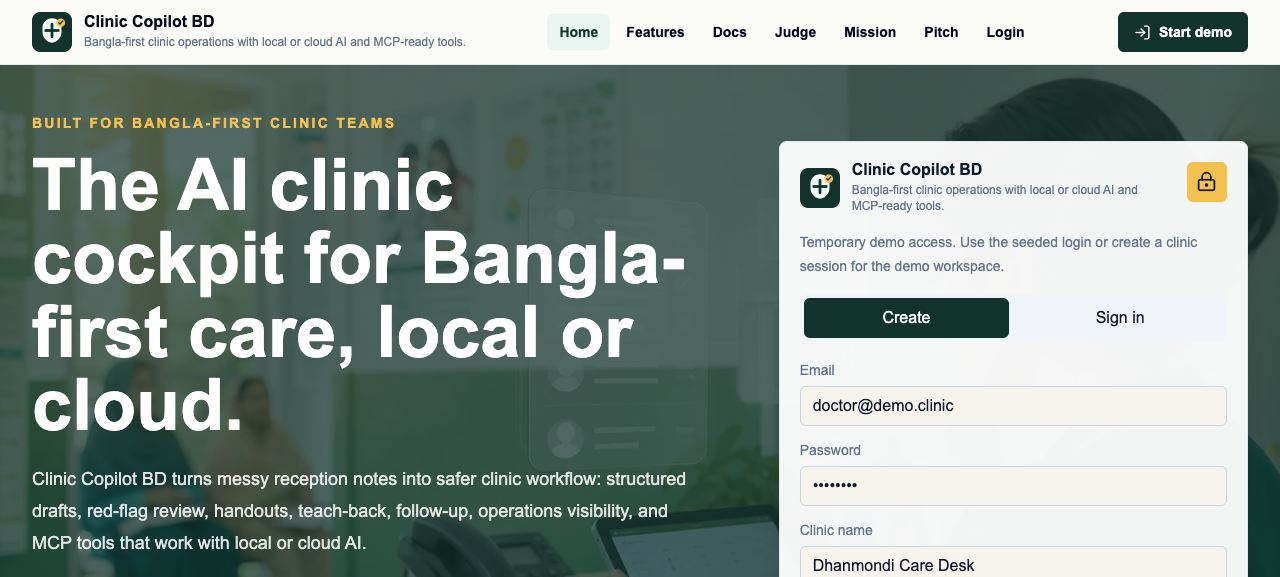
\includegraphics[width=\linewidth]{artifacts/health-worker-latex-main/01-public-home.png}
  \vfill
  \begin{tabularx}{\linewidth}{@{}lY@{}}
    \textbf{Hackathon segment} & Health Worker Assistant: an AI decision-support tool for field health workers to improve frontline healthcare delivery. \\
    \textbf{Audience} & Investors, hospital owners, clinic operators, hackathon judges, healthcare researchers, NGO/public-health partners, and marketing teams. \\
    \textbf{Team} & Huntriox. Lead: Touhidul Alam Seyam. Contact: seyamalam41@gmail.com. \\
    \textbf{Report status} & Live prototype evidence, fresh screenshots, MCP architecture, synthetic-data demo, production hardening plan. \\
    \textbf{Date} & June 12, 2026. \\
  \end{tabularx}
\end{titlepage}
\nopagecolor
\color{clinicInk}

\tableofcontents
\newpage

\section{Executive Summary}

Clinic Copilot BD is a Bangla-first AI workflow assistant for smaller hospitals, private clinics, community clinics, and frontline health workers. It helps a real care team move from a messy patient story to a safer next action without pretending to replace a clinician.

\callout{clinicMint}{
\textbf{Product thesis.} The best health-worker AI for Bangladesh is not the most medically aggressive chatbot. It is the one that reduces workload, catches missing checks, keeps outputs draft-only, works with local or cloud models, and makes human review auditable.
}

\subsection{What the product does}

\begin{enumerate}
  \item Captures intake in Bangla, English, or mixed language.
  \item Converts rough notes into structured draft support.
  \item Flags missing vitals, allergy gaps, pregnancy/child/chest-pain risk, and return-warning blockers.
  \item Produces clinician-reviewable handoff, print packet, patient education, and follow-up tasks.
  \item Keeps an audit trail and requires human review for clinical or patient-facing outputs.
  \item Exposes the same safe workflows through MCP so external agents and local AI hosts can call bounded tools.
\end{enumerate}

\subsection{Primary wedge}

The first commercial wedge is the smaller hospital or overloaded clinic: facilities with heavy patient flow, thin staffing, limited IT capacity, and urgent need for intake, queue, documentation, patient education, and follow-up support.

\subsection{Expansion path}

The same system expands into larger hospitals through outpatient throughput, emergency intake support, nursing handoff, discharge education, quality audit, training, and research evaluation.

\section{Team Huntriox}

\begin{figure}[H]
  \centering
  
\includegraphics[width=1.35in]{artifacts/health-worker-latex-main/huntriox-logo.png}
  \hspace{0.6in}
  
\includegraphics[width=1.2in]{artifacts/health-worker-latex-main/project-logo.svg.png}
  \caption{Team Huntriox and Clinic Copilot BD project identity.}
\end{figure}

\callout{clinicMint}{
\textbf{Team name: Huntriox.} The team combines software engineering, AI product development, and computer engineering perspectives from Bangladesh. The project is led by Touhidul Alam Seyam. Primary contact: \href{mailto:seyamalam41@gmail.com}{seyamalam41@gmail.com}.
}

\membercard
  {Touhidul Alam Seyam}
  {Team Lead}
  {Department of Computer Engineering, BGC Trust University Bangladesh}
  {Also Software Engineer at Agentic AI Institute. Leads product architecture, AI workflow, MCP integration, safety model, and demo execution.}

\membercard
  {Abtahee Kabir}
  {Team Member}
  {Department of Computer Engineering, CUET}
  {Supports engineering, implementation review, technical validation, and hackathon delivery.}

\membercard
  {Chandnin Barua Jowthi}
  {Team Member}
  {Department of Computer Engineering, BGC Trust University Bangladesh}
  {Supports product research, user perspective, healthcare workflow framing, and presentation readiness.}

\section{Fresh Product Screenshots}

The following screenshots were captured from the running app for this PDF report using the project browser QA flow and a focused asset set. They show the main surfaces a judge, buyer, researcher, or investor should inspect.

\screenshot{artifacts/health-worker-latex-main/01-public-home.png}{Public home and product positioning}{The first impression frames Clinic Copilot BD as a practical health worker assistant with local/cloud AI and MCP-ready tools.}

\screenshot{artifacts/health-worker-latex-main/02-judge-mode.png}{Evaluation route}{A compact review path for understanding the queue, case workflow, safety gates, Copilot, and MCP evidence.}

\screenshot{artifacts/health-worker-latex-main/03-docs-mcp.png}{Documentation and MCP proof path}{The docs give technical reviewers a reproducible path through local AI, cloud AI, MCP, and the demo workflow.}

\screenshot{artifacts/health-worker-latex-main/04-live-queue.png}{Live queue workspace}{Queue pressure, red-flag lane, owners, and follow-up status are visible for overloaded front desks.}

\screenshot{artifacts/health-worker-latex-main/05-case-safety-gates.png}{Case workspace and clinical safety gates}{Intake, missing checks, safety gates, draft support, handout, medicine safety, and approval guard are grouped around the patient case.}

\screenshot{artifacts/health-worker-latex-main/06-generated-draft-and-safety.png}{Generated draft and safety workflow}{The app exercises AI generation and safety checks while keeping outputs draft-only.}

\screenshot{artifacts/health-worker-latex-main/07-copilot-receipts-approvals.png}{Copilot, run receipts, and approvals}{Global Ask Copilot connects to AI run receipts and an approvals inbox for auditable human review.}

\screenshot{artifacts/health-worker-latex-main/08-operations-pulse.png}{Operations pulse}{Supervisors can see queue, follow-up, and shift pressure instead of only one patient at a time.}

\screenshot{artifacts/health-worker-latex-main/09-admin-readiness.png}{Admin readiness and governance}{Admin surfaces support readiness, audit, and integration review.}

\screenshot{artifacts/health-worker-latex-main/10-mcp-response.png}{MCP Explorer response}{The MCP Explorer proves that external agents can inspect and call bounded clinic workflow tools.}

\section{Bangladesh Market Context}

Bangladesh is a strong proving ground because frontline delivery pressure is real, physician density is low, out-of-pocket burden is high, and community health worker models already exist.

\begin{table}[H]
\centering
\begin{tabularx}{\linewidth}{@{}L{1.8in}L{1.55in}Y@{}}
\toprule
\textbf{Signal} & \textbf{Data point} & \textbf{Why it matters} \\
\midrule
Population & 173.6 million people in 2024 & Small workflow improvements can affect millions of patient encounters. \\
Physician density & 0.722 physicians per 1,000 people in 2023 & Frontline workers carry a large share of first-contact care and triage. \\
Out-of-pocket burden & 79.3\% of current health expenditure in 2023 & Avoidable revisits, confusion, and missed warning signs are expensive for families. \\
Community clinic model & One community health care provider assisted by two community health workers & The product maps to the team structure used in local clinics. \\
Private facility footprint & A 2021 brief cites 9,529 DGHS-registered private diagnostic centers in 2020 and reports around 11,940 private hospitals, clinics, and diagnostic centers & Small private facilities are a large fragmented market for lightweight workflow software. \\
Digital strategy alignment & Bangladesh Digital Health Strategy 2023-2027 emphasizes mHealth, AI, interoperability, privacy, and service innovation & The project fits national direction, not just hackathon novelty. \\
\bottomrule
\end{tabularx}
\end{table}

\section{Global Healthcare Constraints}

The same pressures visible in Bangladesh are part of a wider global pattern: too few health workers, incomplete access to essential services, high out-of-pocket exposure, and frontline teams that need practical support rather than another generic chatbot.

\begin{table}[H]
\centering
\begin{tabularx}{\linewidth}{@{}L{1.9in}L{1.85in}Y@{}}
\toprule
\textbf{Constraint} & \textbf{Global signal} & \textbf{Why this supports the project} \\
\midrule
Health worker shortage & WHO estimates a projected shortfall of 11 million health workers by 2030, mostly in low- and lower-middle-income countries. & Decision support must help scarce staff work safely, not assume more doctors are immediately available. \\
Essential service gaps & WHO and World Bank estimate that about 4.6 billion people were not fully covered by essential health services in 2023. & Frontline and primary-care workflows need tools that improve access, triage, education, and follow-up at the first point of care. \\
Financial hardship & WHO reports that 2.1 billion people faced financial hardship from health expenses in 2022, including 1.6 billion people living in or pushed deeper into poverty. & Reducing avoidable revisits, missed warning signs, and unclear instructions has direct household value. \\
Low physician density & World Bank physician-density data shows low-income countries at roughly 0.4 physicians per 1,000 people and lower-middle-income countries around 0.7 in 2022. & The product is designed for nurse, CHW, reception, and clinician teamwork in settings where physician time is limited. \\
Need for digital job aids & Digital health literature highlights training, communication, job aids, supervision, and decision support as useful roles for technology in low-resource health workforces. & Clinic Copilot BD is a bounded workflow assistant: it supports staff tasks, safety checks, handoff, and education without claiming autonomous medical authority. \\
\bottomrule
\end{tabularx}
\end{table}

\section{Primary Market: Smaller Hospitals and Overloaded Clinics}

The highest-probability first buyer is not a highly resourced tertiary hospital. It is the smaller hospital, local private clinic, diagnostic-linked clinic, NGO clinic, community clinic, or busy outpatient desk where staff are stretched and the workflow is still paper-heavy.

\subsection{Why smaller facilities feel the pain first}

\begin{itemize}
  \item One doctor may cover too many patients.
  \item Nurses often handle intake, triage, patient explanation, and coordination at the same time.
  \item Reception staff may capture symptoms without a clinical checklist.
  \item Paper notes, WhatsApp follow-up, printed slips, and verbal handoff are fragmented.
  \item Patients may return because instructions were unclear.
  \item High-risk cases can wait in the same queue as routine cases.
  \item Staff turnover makes consistent protocols hard to maintain.
\end{itemize}

\subsection{How Clinic Copilot BD helps}

\begin{table}[H]
\centering
\begin{tabularx}{\linewidth}{@{}L{2.3in}Y@{}}
\toprule
\textbf{Operational pain} & \textbf{Product response} \\
\midrule
Too many patients for the available doctor & Queue risk summary, red-flag lane, missing-vitals checks, concise doctor handoff. \\
Reception captures incomplete information & Bangla/English intake cleanup, missing question finder, safety gate prompts. \\
Nurses are overloaded & Staff task list, vitals/allergy blockers, approval readiness, visit closeout checklist. \\
Patient education takes time & Simple Bangla handout, teach-back checklist, audio script, pictogram plan. \\
Follow-up is inconsistent & Follow-up due panel, call sheet, reply triage, owner badges. \\
Documentation slows the visit & Draft SOAP support, referral packet, print workflow, AI run receipt. \\
Clinic owner needs quality visibility & Audit log, operations pulse, trends, MCP resource access. \\
\bottomrule
\end{tabularx}
\end{table}

\section{Larger Hospital Benefit}

Large hospitals have more staff, but they still face bottlenecks in OPD, emergency intake, nursing handoff, patient education, and quality review.

\begin{table}[H]
\centering
\begin{tabularx}{\linewidth}{@{}L{2.1in}Y@{}}
\toprule
\textbf{Area} & \textbf{Benefit} \\
\midrule
Outpatient department & Faster intake normalization, risk sorting, and doctor-ready summaries. \\
Emergency or urgent desk & Conservative red-flag prompts and escalation blockers before patients wait too long. \\
Nursing stations & Shared task list, handoff, visit closeout, and approval readiness. \\
Discharge and patient education & Simple Bangla instructions, teach-back, return warnings, and follow-up ownership. \\
Training & Synthetic scenarios, scorecards, role-based practice, and reviewable AI run receipts. \\
Quality and compliance & Audit trail, safety envelope, approval logs, and MCP-readable workflow outputs. \\
Research and evaluation & Structured case scenarios, measurable outputs, and reproducible MCP tool calls. \\
\bottomrule
\end{tabularx}
\end{table}

\section{Workflow Design}

\subsection{Field-to-clinic loop}

\begin{center}
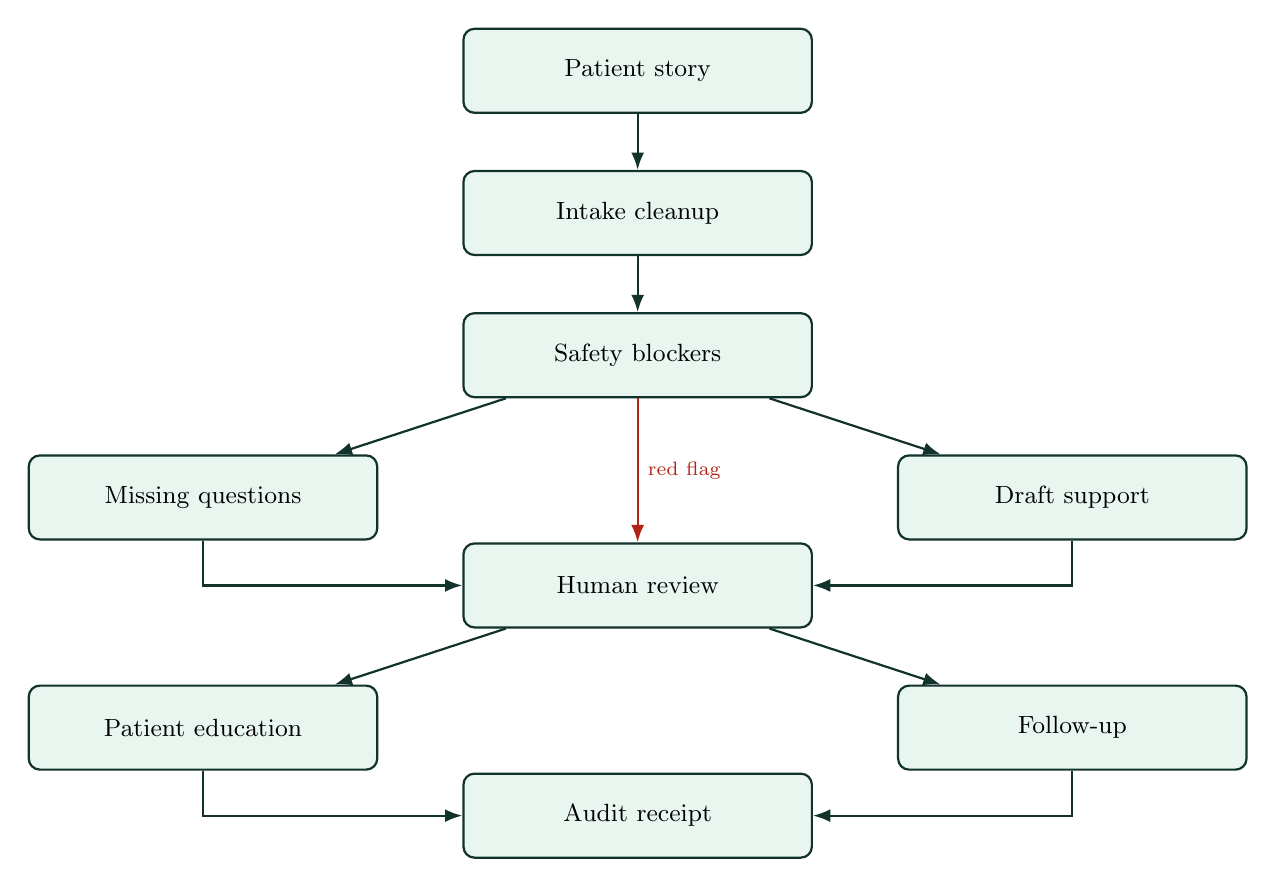
\begin{tikzpicture}[
  node distance=0.28in and 0.42in,
  box/.style={rectangle,rounded corners,draw=clinicGreen,fill=clinicMint,thick,align=center,minimum height=0.42in,text width=1.65in,font=\small},
  arrow/.style={-{Latex[length=2.2mm]},thick,color=clinicGreen}
]
\node[box] (a) {Patient story};
\node[box,below=of a] (b) {Intake cleanup};
\node[box,below=of b] (c) {Safety blockers};
\node[box,below left=of c] (d) {Missing questions};
\node[box,below right=of c] (e) {Draft support};
\node[box,below=0.72in of c] (f) {Human review};
\node[box,below left=of f] (g) {Patient education};
\node[box,below right=of f] (h) {Follow-up};
\node[box,below=0.72in of f] (i) {Audit receipt};
\draw[arrow] (a) -- (b);
\draw[arrow] (b) -- (c);
\draw[arrow] (c) -- (d);
\draw[arrow] (c) -- (e);
\draw[arrow] (d) |- (f);
\draw[arrow] (e) |- (f);
\draw[arrow] (f) -- (g);
\draw[arrow] (f) -- (h);
\draw[arrow] (g) |- (i);
\draw[arrow] (h) |- (i);
\draw[arrow,color=clinicDanger] (c) -- node[right,font=\scriptsize,color=clinicDanger]{red flag} (f);
\end{tikzpicture}
\end{center}

\subsection{Multi-role workflow}

\begin{table}[H]
\centering
\begin{tabularx}{\linewidth}{@{}L{1.6in}L{2in}Y@{}}
\toprule
\textbf{Viewpoint} & \textbf{Main need} & \textbf{Product surface} \\
\midrule
Reception & Capture story quickly & Intake, queue, command copilot. \\
Community health worker & Ask what matters next & Safety blockers, missing questions, patient education. \\
Nurse & Confirm safety gates & Vitals/allergy/return-warning checks, handoff. \\
Doctor & Review concise support & SOAP support, risk explanation, approval readiness. \\
Follow-up desk & Close the loop & Scheduler, reply triage, due panel. \\
Admin/program manager & See service delivery & Trends, audit logs, queue pressure, MCP resources. \\
External agent & Integrate safely & MCP stdio server and HTTP demo endpoint. \\
\bottomrule
\end{tabularx}
\end{table}

\section{AI Safety Architecture}

\subsection{Allowed AI behavior}

\begin{itemize}
  \item Summarize intake.
  \item Suggest missing questions.
  \item Draft handoff notes.
  \item Draft patient education.
  \item Flag safety blockers.
  \item Prepare review packets.
  \item Explain risk uncertainty.
  \item Suggest operational next steps.
\end{itemize}

\subsection{Disallowed AI behavior}

\begin{itemize}
  \item Diagnose.
  \item Prescribe.
  \item Approve final care.
  \item Dismiss urgent symptoms.
  \item Finalize patient-facing instructions without human review.
  \item Replace clinicians.
\end{itemize}

\subsection{Safety control flow}

\begin{center}
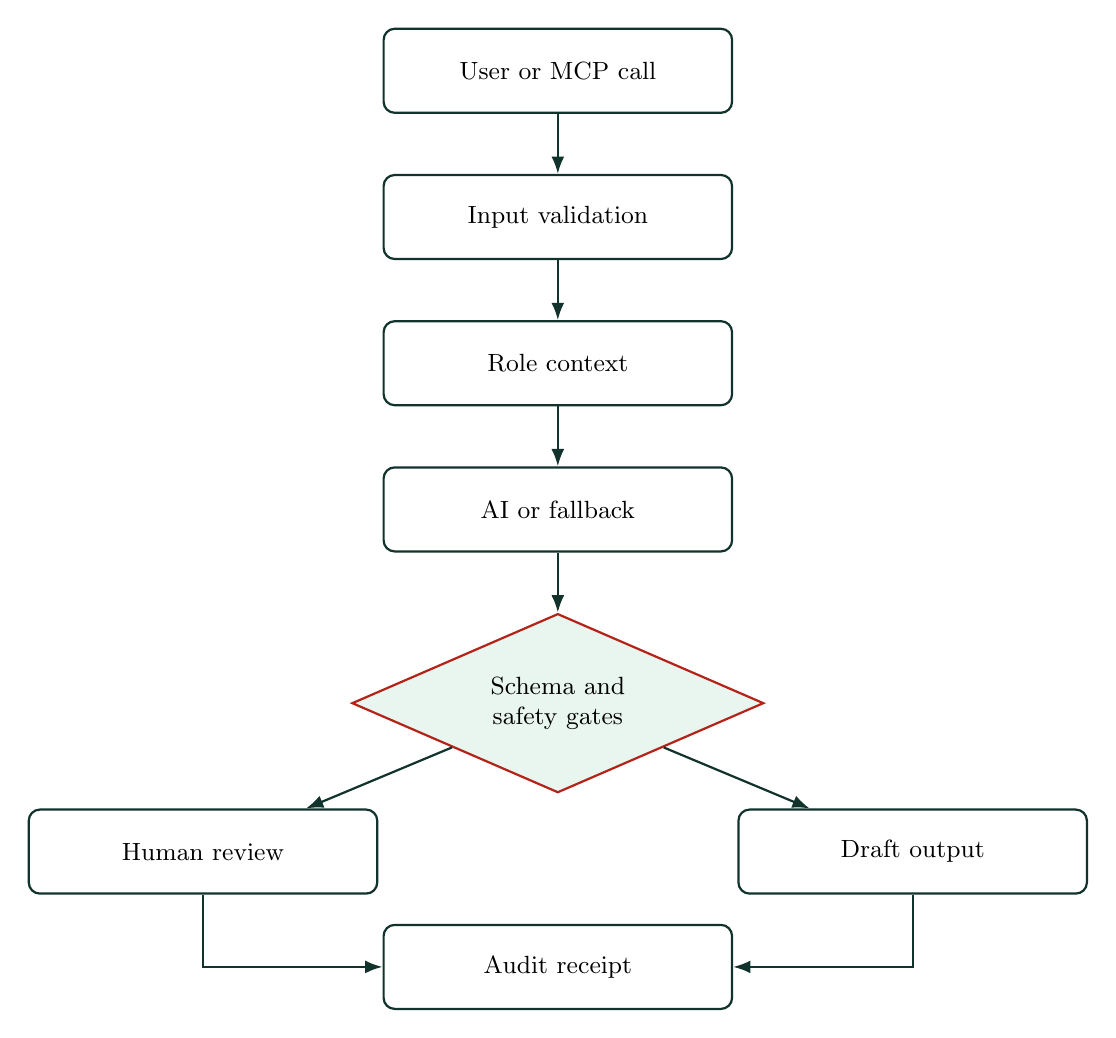
\begin{tikzpicture}[
  node distance=0.3in and 0.38in,
  box/.style={rectangle,rounded corners,draw=clinicGreen,fill=white,thick,align=center,minimum height=0.42in,text width=1.65in,font=\small},
  guard/.style={diamond,aspect=2.3,draw=clinicDanger,fill=clinicMint,thick,align=center,text width=1.15in,font=\small},
  arrow/.style={-{Latex[length=2.2mm]},thick,color=clinicGreen}
]
\node[box] (a) {User or MCP call};
\node[box,below=of a] (b) {Input validation};
\node[box,below=of b] (c) {Role context};
\node[box,below=of c] (d) {AI or fallback};
\node[guard,below=of d] (e) {Schema and safety gates};
\node[box,below left=of e] (f) {Human review};
\node[box,below right=of e] (g) {Draft output};
\node[box,below=0.65in of e] (h) {Audit receipt};
\draw[arrow] (a) -- (b);
\draw[arrow] (b) -- (c);
\draw[arrow] (c) -- (d);
\draw[arrow] (d) -- (e);
\draw[arrow] (e) -- (f);
\draw[arrow] (e) -- (g);
\draw[arrow] (f) |- (h);
\draw[arrow] (g) |- (h);
\end{tikzpicture}
\end{center}

\section{Security Model}

Clinic Copilot BD is currently a hackathon prototype using synthetic data and temporary demo authentication. The production security model is designed around patient privacy, role boundaries, model governance, and auditability.

\subsection{Current prototype boundaries}

\begin{itemize}
  \item Synthetic demo data only.
  \item Temporary demo login for testing.
  \item AI outputs are draft support, not final clinical authority.
  \item MCP tools return safety envelopes.
  \item API routes validate inputs and fall back to safe deterministic responses.
  \item No production PHI storage claim is made in the demo.
\end{itemize}

\subsection{Production hardening plan}

\begin{table}[H]
\centering
\begin{tabularx}{\linewidth}{@{}L{1.65in}Y@{}}
\toprule
\textbf{Layer} & \textbf{Production control} \\
\midrule
Identity & Real organization accounts, SSO/OIDC where available, and role-based access for reception, nurse, clinician, admin, auditor, and researcher. \\
Authorization & Server-side role checks for every case, tool call, approval, export, and patient-facing output. No client-trusted user IDs. \\
Patient data & Encryption in transit, encryption at rest, tenant isolation, minimal retention, consent flow, and configurable data residency. \\
Local AI & LM Studio or local OpenAI-compatible models can run inside the clinic/hospital network for privacy-sensitive deployments. \\
Cloud AI & Cloud calls use redaction, minimum necessary context, provider allowlist, timeout, schema validation, and audit logging. \\
MCP & Tool allowlist, server-side validation, role-scoped outputs, safety envelopes, and no MCP bypass of clinic permissions. \\
Audit & Immutable event trail for intake changes, AI calls, approvals, print packets, exports, and MCP calls. \\
Human review & Patient-facing instructions, clinical handoffs, referrals, and signoff packets remain drafts until a responsible staff member approves. \\
Research mode & De-identified exports, synthetic scenarios, scenario scorecards, and reproducible tool calls before real-world studies. \\
Operations & Rate limits, monitoring, error reporting, backup/restore, incident response, and admin controls for disabling model providers or tools. \\
\bottomrule
\end{tabularx}
\end{table}

\subsection{Security architecture}

\begin{center}
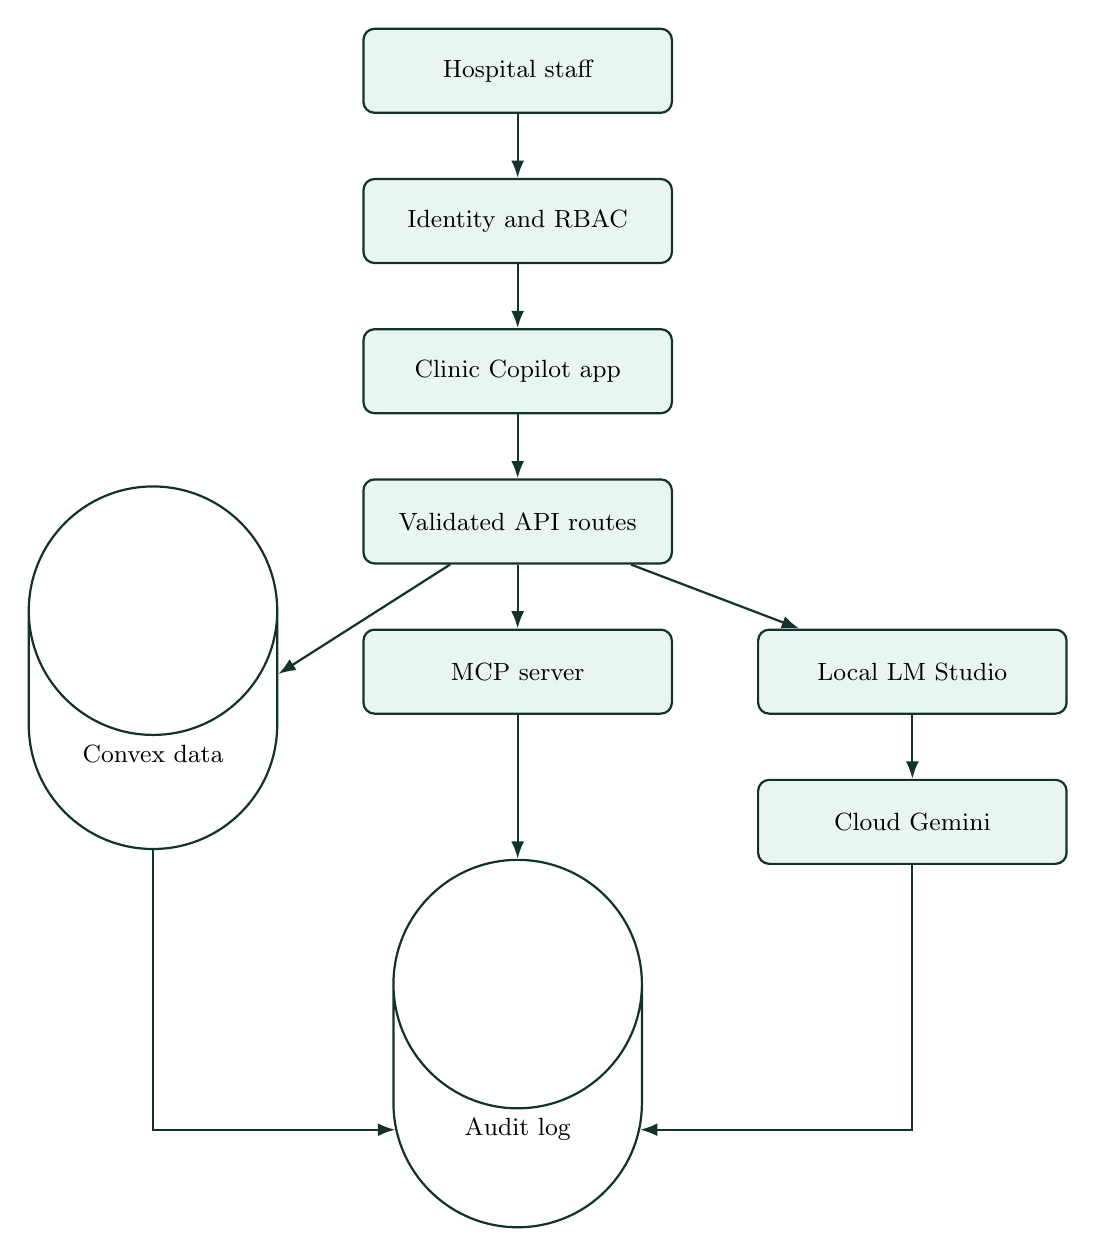
\begin{tikzpicture}[
  node distance=0.32in and 0.42in,
  box/.style={rectangle,rounded corners,draw=clinicGreen,fill=clinicMint,thick,align=center,minimum height=0.42in,text width=1.45in,font=\small},
  store/.style={cylinder,shape border rotate=90,draw=clinicGreen,fill=white,thick,align=center,minimum height=0.42in,text width=1.15in,font=\small},
  arrow/.style={-{Latex[length=2.2mm]},thick,color=clinicGreen}
]
\node[box] (u) {Hospital staff};
\node[box,below=of u] (auth) {Identity and RBAC};
\node[box,below=of auth] (app) {Clinic Copilot app};
\node[box,below=of app] (api) {Validated API routes};
\node[store,below left=of api] (db) {Convex data};
\node[box,below=of api] (mcp) {MCP server};
\node[box,below right=of api] (local) {Local LM Studio};
\node[box,below=of local] (cloud) {Cloud Gemini};
\node[store,below=0.72in of mcp] (audit) {Audit log};
\draw[arrow] (u) -- (auth);
\draw[arrow] (auth) -- (app);
\draw[arrow] (app) -- (api);
\draw[arrow] (api) -- (db);
\draw[arrow] (api) -- (mcp);
\draw[arrow] (api) -- (local);
\draw[arrow] (local) -- (cloud);
\draw[arrow] (db) |- (audit);
\draw[arrow] (mcp) -- (audit);
\draw[arrow] (cloud) |- (audit);
\end{tikzpicture}
\end{center}

\section{MCP Strategy}

MCP turns Clinic Copilot BD from a standalone app into an agent-ready health workflow layer.

\subsection{What MCP enables}

\begin{itemize}
  \item LM Studio can call clinic tools from local models.
  \item Claude, Codex, Cursor-style clients, and other MCP hosts can spawn the stdio MCP server.
  \item Public demos can call \texttt{/api/mcp} over JSON-RPC.
  \item External agents can inspect tool schemas before acting.
  \item Safety rules travel with tool outputs.
\end{itemize}

\subsection{MCP tools}

\begin{verbatim}
clinic.demo_manifest
clinic.list_demo_scenarios
clinic.workflow_brief
clinic.tools.list
clinic.tools.describe
clinic.queue.snapshot
clinic.safety.get_blockers
clinic.print.prepare_packet
clinic.literacy.prepare
clinic.sync.preview_queue
clinic.approval.request
clinic.demo.score_scenario
\end{verbatim}

\subsection{MCP resources}

\begin{verbatim}
clinic://demo/scenarios
clinic://demo/capabilities
clinic://agents/tool-registry
clinic://safety/gates
\end{verbatim}

\section{Local and Cloud Model Strategy}

\subsection{Why local models matter}

Field settings may have unstable internet, privacy concerns, low budget, latency constraints, limited cloud availability, and model vendor uncertainty. Clinic Copilot BD supports LM Studio locally through the AI SDK OpenAI-compatible provider.

\subsection{Why cloud models matter}

Cloud models can provide stronger structured output, better multilingual reasoning, easier scaling during pilots, and centralized model updates. Clinic Copilot BD supports Google Gemini through \texttt{@ai-sdk/google}.

\subsection{Why fallback matters}

For demonstrations, training, and offline-style use, the app can return safe deterministic output when no provider is configured. This makes the product testable without fragile API dependencies.

\subsection{Deployment pattern}

\begin{center}
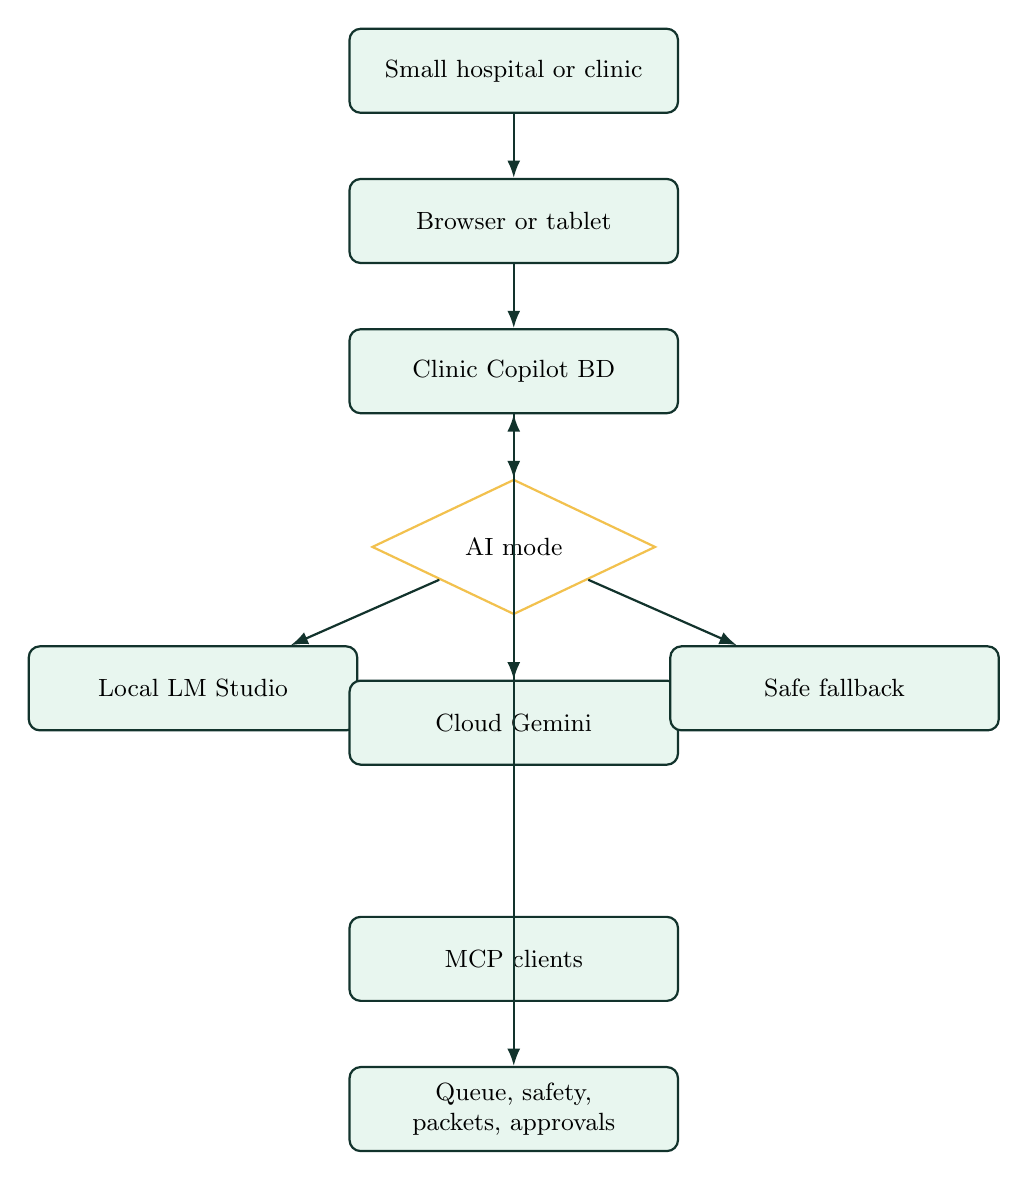
\begin{tikzpicture}[
  node distance=0.32in and 0.42in,
  box/.style={rectangle,rounded corners,draw=clinicGreen,fill=clinicMint,thick,align=center,minimum height=0.42in,text width=1.55in,font=\small},
  choice/.style={diamond,aspect=2.1,draw=clinicGold,fill=white,thick,align=center,text width=0.95in,font=\small},
  arrow/.style={-{Latex[length=2.2mm]},thick,color=clinicGreen}
]
\node[box] (facility) {Small hospital or clinic};
\node[box,below=of facility] (browser) {Browser or tablet};
\node[box,below=of browser] (app) {Clinic Copilot BD};
\node[choice,below=of app] (mode) {AI mode};
\node[box,below left=of mode] (local) {Local LM Studio};
\node[box,below=of mode] (cloud) {Cloud Gemini};
\node[box,below right=of mode] (fallback) {Safe fallback};
\node[box,below=0.75in of cloud] (mcp) {MCP clients};
\node[box,below=of mcp] (tools) {Queue, safety, packets, approvals};
\draw[arrow] (facility) -- (browser);
\draw[arrow] (browser) -- (app);
\draw[arrow] (app) -- (mode);
\draw[arrow] (mode) -- (local);
\draw[arrow] (mode) -- (cloud);
\draw[arrow] (mode) -- (fallback);
\draw[arrow] (mcp) -- (app);
\draw[arrow] (app) -- (tools);
\end{tikzpicture}
\end{center}

\section{Feature Inventory}

\subsection{AI workflow}

\begin{itemize}
  \item Local LM Studio provider, cloud Google Gemini provider, and no-key deterministic fallback.
  \item Mixed Bangla/English intake cleanup, clinical draft generation, SOAP-style support, and missing question finder.
  \item Current-case AI Q\&A, command copilot, draft edit support, document extraction, clinic briefing, and next-step navigator.
\end{itemize}

\subsection{Safety}

\begin{itemize}
  \item Red-flag summary, vitals requirement checks, allergy gap checks, and medicine clarity checker.
  \item Pregnancy, child, and chest-pain escalation patterns plus approval readiness guard and visit closeout checklist.
  \item Risk explanation, human-review boundary, AI run receipts, approvals inbox, and audit log viewer.
\end{itemize}

\subsection{Health worker operations}

Queue board; waiting-time labels; red-flag lane; staff owner badges; follow-up due panel; operations pulse; shift copilot; staff handoff; trend dashboard; low-connectivity review queue; role-aware workspaces.

\subsection{Patient communication}

Bangla/English handout; printable handout; medicine slip; referral packet; doctor summary; follow-up call sheet; simple Bangla mode; pictogram support; audio script support; teach-back checklist; patient question answer assistant; reply triage; follow-up composer and scheduler.

\subsection{Agentic and MCP layer}

Stdio MCP server; HTTP JSON-RPC demo endpoint; MCP tools/list and resources/read; \texttt{mcp.json} for LM Studio and local MCP hosts; MCP Explorer in Admin; tool registry resource; safety gate resource; demo scenario resource; capability map resource; scenario scorecard.

\section{Stack, Scalability, and Modularity}

\begin{table}[H]
\centering
\begin{tabularx}{\linewidth}{@{}L{1.7in}Y@{}}
\toprule
\textbf{Layer} & \textbf{Technology} \\
\midrule
Frontend & Next.js 16 App Router, React 19, TypeScript. \\
Styling & Tailwind CSS 4, responsive mobile-first UI. \\
Backend & Convex realtime data, Next.js API routes. \\
AI SDK & Vercel AI SDK 6. \\
Cloud AI & \texttt{@ai-sdk/google}. \\
Local AI & \texttt{@ai-sdk/openai-compatible} for LM Studio. \\
MCP & \texttt{@modelcontextprotocol/sdk}, stdio server, JSON-RPC HTTP demo route. \\
Validation & Zod schemas. \\
QA & Bun tests, Biome, Next build, browser QA, MCP smoke. \\
Runtime & Bun. \\
\bottomrule
\end{tabularx}
\end{table}

\subsection{Scalable rollout path}

\begin{enumerate}
  \item Demo mode with synthetic cases.
  \item Small hospital or clinic pilot with no real patient storage.
  \item Community clinic or NGO pilot with supervised health workers.
  \item Local LM Studio deployment for privacy-sensitive training.
  \item Cloud provider deployment for stronger model quality.
  \item Convex-backed realtime case workflow.
  \item MCP integration with health system tools and NGO dashboards.
\end{enumerate}

\section{Why Investors Should Care}

\begin{enumerate}
  \item \textbf{The pain is operational, frequent, and expensive.} Every clinic day creates repeated intake, triage, documentation, education, follow-up, and handoff work.
  \item \textbf{Smaller hospitals are a practical wedge.} They need immediate workload relief without buying a heavy hospital information system.
  \item \textbf{Bangladesh is a high-leverage proving ground.} Large population, low physician density, strong CHW history, high household spending burden, and national digital health priorities create a strong reason to test here.
  \item \textbf{The product avoids the riskiest AI-health trap.} It does not sell autonomous diagnosis. It sells decision support, documentation acceleration, safety checks, and human-reviewed patient communication.
  \item \textbf{The architecture is model-flexible.} Local and cloud AI support reduces vendor lock-in and supports low-resource deployment.
  \item \textbf{MCP makes it platform-shaped.} The app can become a safe tool layer for other agents, not just a standalone UI.
\end{enumerate}

\subsection{Investor wedge}

\begin{center}
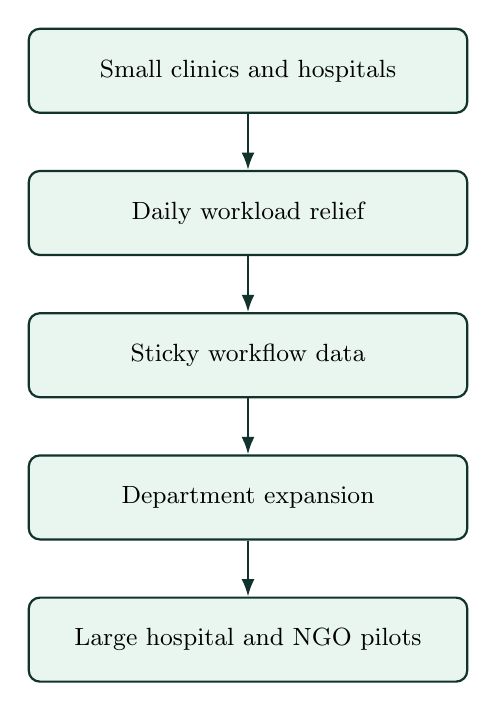
\begin{tikzpicture}[
  node distance=0.28in,
  box/.style={rectangle,rounded corners,draw=clinicGreen,fill=clinicMint,thick,align=center,minimum height=0.42in,text width=2.1in,font=\small},
  arrow/.style={-{Latex[length=2.2mm]},thick,color=clinicGreen}
]
\node[box] (a) {Small clinics and hospitals};
\node[box,below=of a] (b) {Daily workload relief};
\node[box,below=of b] (c) {Sticky workflow data};
\node[box,below=of c] (d) {Department expansion};
\node[box,below=of d] (e) {Large hospital and NGO pilots};
\draw[arrow] (a) -- (b);
\draw[arrow] (b) -- (c);
\draw[arrow] (c) -- (d);
\draw[arrow] (d) -- (e);
\end{tikzpicture}
\end{center}

\section{Validation Proof}

\begin{itemize}
  \item The refreshed screenshot run completed from a production build through public pages, authenticated workspace, AI actions, drawer views, and MCP Explorer.
  \item The app is currently reachable at \texttt{http://localhost:3000}.
  \item The screenshot command used a temporary server on port \texttt{3003} and saved focused report images into the LaTeX asset folder.
  \item PDF compilation uses \texttt{tectonic}.
\end{itemize}

\section{Risks and Honest Limitations}

\begin{table}[H]
\centering
\begin{tabularx}{\linewidth}{@{}L{2.35in}Y@{}}
\toprule
\textbf{Risk} & \textbf{Current mitigation} \\
\midrule
Local models may return invalid structured JSON & Timeout, no-retry setting, provider failure fallback, schema tests. \\
AI could be mistaken for medical authority & Product copy, prompts, safety envelopes, human-review flags, approval inbox. \\
Connectivity may be weak & Demo fallback and low-connectivity review queue pattern. \\
Real deployment needs privacy/security hardening & Current demo uses synthetic data and temporary auth only. \\
Field UX must be tested with real CHWs and clinic staff & Current app is a prototype; next step is supervised usability testing. \\
\bottomrule
\end{tabularx}
\end{table}

\section{Next Milestones}

\begin{enumerate}
  \item Add explicit provider status in the UI: local live, cloud live, fallback, timeout.
  \item Build offline-first Android wrapper or PWA field mode.
  \item Add maternal/child/NCD-specific field protocols.
  \item Add supervisor dashboard for CHW and small-hospital programs.
  \item Add exportable program reports.
  \item Add privacy hardening and production authentication.
  \item Pilot with synthetic or anonymized workflows before any real patient use.
\end{enumerate}

\section{Source Notes}

\begin{itemize}
  \item World Bank Open Data, Bangladesh population: 173,562,364 in 2024. \href{https://data.worldbank.org/indicator/SP.POP.TOTL?locations=BD}{World Bank population indicator}.
  \item World Bank Open Data, physicians per 1,000 people: 0.722 in 2023. \href{https://data.worldbank.org/indicator/SH.MED.PHYS.ZS?locations=BD}{World Bank physicians indicator}.
  \item World Bank Open Data, out-of-pocket expenditure share of current health expenditure: 79.30711365\% in 2023. \href{https://data.worldbank.org/indicator/SH.XPD.OOPC.CH.ZS?locations=BD}{World Bank out-of-pocket expenditure indicator}.
  \item WHO and World Bank Universal Health Coverage reporting: about 4.6 billion people not fully covered by essential services in 2023, and 2.1 billion people facing financial hardship from health expenses in 2022. \href{https://www.who.int/news-room/fact-sheets/detail/universal-health-coverage-\%28uhc\%29}{WHO UHC fact sheet}.
  \item WHO health workforce topic page: projected shortfall of 11 million health workers by 2030, mostly in low- and lower-middle-income countries. \href{https://www.who.int/health-topics/health-workforce}{WHO health workforce}.
  \item BMJ Global Health reassessment of global workforce shortage: 15 million health workers in 2020 decreasing to 10 million by 2030. \href{https://gh.bmj.com/content/7/6/e009316}{BMJ Global Health workforce study}.
  \item World Bank Open Data physicians indicator showing low-income and lower-middle-income physician density by income group. \href{https://data.worldbank.org/indicator/SH.MED.PHYS.ZS}{World Bank global physicians indicator}.
  \item WHO feature story on Bangladesh community health workers and community clinics. \href{https://www.who.int/news-room/feature-stories/detail/bangladesh-community-health-workers-at-the-heart-of-a-stronger-health-system-and-the-fight-against-covid-19}{WHO Bangladesh CHW story}.
  \item CHW Central profile of BRAC Shasthya Shebika and Shasthya Kormi programs. \href{https://chwcentral.org/the-brac-shasthya-shebika-and-shasthya-kormi-community-health-workers-in-bangladesh/}{CHW Central BRAC profile}.
  \item Frontline Health Workers Coalition article citing Shasthya Shebika scale and maternal health reach. \href{https://www.frontlinehealthworkers.org/blog/weve-made-staggering-progress-maternal-health-bangladesh-where-next}{Frontline Health Workers Coalition article}.
  \item Data for Impact brief on private health care data collection in Bangladesh. \href{https://www.data4impactproject.org/wp-content/uploads/2021/05/Improving-Private-Health-Care-Data-Collection_fs-21-517_d4i-1.pdf}{Data for Impact Bangladesh private healthcare brief}.
  \item Human Resources for Health article on Bangladesh health workforce crisis. \href{https://pmc.ncbi.nlm.nih.gov/articles/PMC3037300/}{Bangladesh health workforce crisis article}.
  \item PLOS ONE study on working conditions of clinical health workers in Bangladesh primary and secondary healthcare facilities. \href{https://journals.plos.org/plosone/article?id=10.1371/journal.pone.0294224}{PLOS ONE working conditions study}.
  \item Bangladesh Digital Health Strategy 2023-2027 summary. \href{https://dig.watch/resource/the-bangladesh-digital-health-strategy-2023-2027}{Bangladesh Digital Health Strategy summary}.
  \item Digital health intervention study in Bangladesh using community health workers, smart health kit, AI-based mobile app, household visits, risk assessment, and digital referrals. \href{https://link.springer.com/article/10.1186/s12889-025-22770-9}{BMC Public Health digital health intervention study}.
  \item Johns Hopkins Center for Global Digital Health Innovation overview of digital strategies for frontline workers, including job aids, supervision, communication, and data for decision-making. \href{https://publichealth.jhu.edu/center-for-global-digital-health-innovation/digital-strategies-for-frontline-workers-delivering-child-health}{Johns Hopkins frontline worker digital strategies}.
\end{itemize}

\end{document}
